\documentclass{beamer}
\usetheme{Warsaw}
\usepackage{polski}
\usepackage[utf8]{inputenc}
\usepackage[T1]{fontenc}
\usepackage{lmodern}
\usepackage{parskip}
\usepackage{graphics}
\usepackage{algorithm}
\usepackage{algpseudocode}
\usepackage{mathtools}

\author{Przemysław Pastuszka}
\institute{Instytut Informatyki UWr}
\date{\today}
\title{Flow Shop Problem}

\makeatletter
\def\verbatim@font{\ttfamily\footnotesize}
\makeatother


\begin{document}

\frame{
    \titlepage
}


\begin{frame}
    \frametitle{Przypomnienie problemu}
    \begin{block}{Dane wejściowe}
        $J$ - zbiór prac do wykonania \\
        $J = \{j^{(0)}, j^{(1)}, \ldots, j^{(n)}\}$ \\
        $M$ - zbiór maszyn \\
        $M = \{m^{(0)}, m^{(1)}, \ldots, m^{(k)}\}$ \\
        $f: J \times M \rightarrow \mathbb{R}$ - funkcja opisująca czasy wykonania zadań na maszynach
    \end{block}
    \end{frame}

\begin{frame}
\frametitle{Przypomnienie problemu}
        \begin{block}{Założenia}
                \begin{itemize}
          \item wszystkie prace muszą zostać wykonane
          \item każda z prac jest wykonywana kolejno na maszynach od $m^{(0)}$ do $m^{(k)}$
          \item maszyna może wykonywać co najwyżej jedno zadanie w danym momencie
        \end{itemize}
    \end{block}
    \pause
    \begin{block}{Nasz cel}
        Znaleźć taką permutację $J$, że łączny czas wykonania wszystkich zadań jest jak najmniejszy.
    \end{block}
\end{frame}

\begin{frame}
    \frametitle{Testowane algorytmy}
        \begin{itemize}
          \item CDS
          \item NEH
          \item algorytm genetyczny
        \end{itemize}
\end{frame}

\begin{frame}
    \frametitle{Szczegóły algorytmu genetycznego}
        \begin{itemize}
          \item chromosom jest permutacją
          \item mutacja zamienia miejscami elementy permutacji
          \item krzyżowanie za pomocą PMX
          \item rodzice wybierani metodą turniejową
          \item elitism
        \end{itemize}
\end{frame}

\begin{frame}
    \frametitle{Wyniki}
    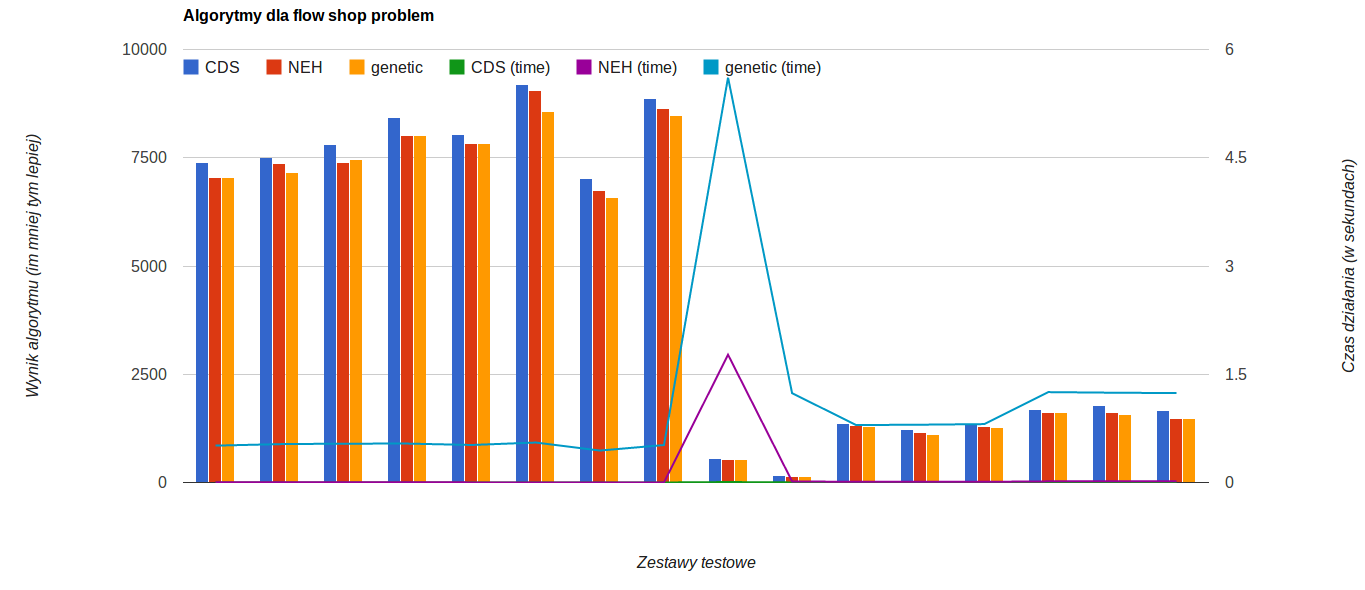
\includegraphics[scale=0.24]{chart.png}
\end{frame}

\begin{frame}
    \frametitle{Implemetacja}
        Cały kod można znaleźć na stronie: \textit{http://github.com/rtshadow/flowshop}
\end{frame}

\end{document}
